\chapter{Codebase: Object Tree}

The object tree is contained within the global wdat object at
wdat.objecttree.

\section{Description}

The object tree is (usually) the first point of user contact after the
login process.  This involves selecting the type of container elements
to be displayed.  Say Blocks were to be selected as the container
element to display the tree by.  This would download all blocks owned
by the user, without datafiles, and display them in the tree.

Now, the user will select one of the blocks.  This will cause two
things to happen:

\begin{enumerate}
  \item
  object tree will update the child node of the selected item by
  downloading its children via the network resources. This update will
  only contain containers.  There is no point showing plottables in
  the object tree since it doesn't offer any functions for plottables.

  \item
  object tree will fire a 'ContainerSelected' event into the WDAT
  event bus.  This event will contain the internal id of the selected
  item.  This allows other parts of the application to update
  themselves as required. 
\end{enumerate}

Clicking on the now loaded children also has the same effects.

Once a particular type of container elements is being viewed, changing
the container type via the selection box will cause the entire list to
be cleared and the new type of containers to be fetched and shown.

\begin{figure}[h!t]
  \centering
  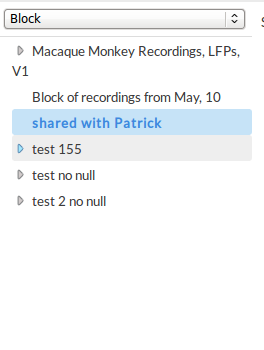
\includegraphics[scale=1.0]{src/images/wdat-object-tree.png}
  \caption{ObjectTree: Note how there is a field to select the type of container objects to show in the list.  Selected items are highlighted in blue.  Items being hovered over are highlighted in lightgrey.  Also, this is a hierarchial tree and child elements are indented to the right. }
\end{figure}

\section{Methods}

There are a few methods exposed by the wdat.objecttree module.

\begin{enumerate}
  \item{wdat.objecttree.add()} \hfill \\
  Add items to the tree interface, and also to the internal state
  variables.

  \item{wdat.objecttree.clear()} \hfill \\
  Clear all items from the tree.  Clears the internal state
  representation as well. 

  \item{wdat.objecttree.remove()} \hfill \\
  Removes specified item from the interface and also from the internal
  state variables.

  \item{wdat.objecttree.setLeaf()} \hfill \\
  Sets the specified node as a leaf.  This changes some graphic
  elements making it seem like there are no children to that
  particular node.
\end{enumerate}
